\section{RedBlack Tree}
I RB-Tree sono ABR i cui nodi hanno un bit extra riservato ad un campo colore $x.color$, che può essere: $red$ per il rosso, $black$ per il nero. \\~\\
Un RB-Tree soddisfa le seguenti proprietà:
\begin{itemize}
    \item Proprietà RB: ogni nodo è colorato, rosso o nero
    \item Proprietà della radice: la radice è nera
    \item Proprietà delle foglie: ogni foglia (NULL) è nera
    \item Proprietà del rosso: se un nodo rosso ha dei figli, questi sono sempre neri
    \item Proprietà Depth: per ogni nodo, qualsiasi percorso semplice da questo nodo a qualsiasi foglia discendente ha la stessa profondità nera (il numero di nodi neri)
\end{itemize}
\begin{center}
    \begin{tabular}{c}
        \\ 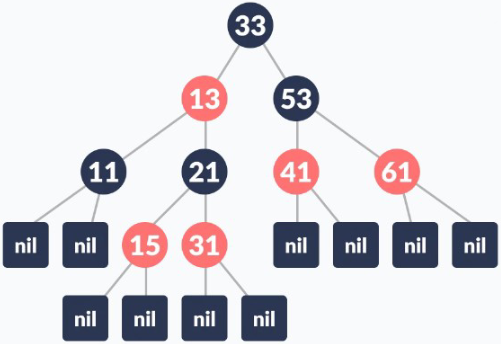
\includegraphics[width=0.7\textwidth]{image/RB-Tree.png} \\ \\
    \end{tabular}
\end{center}
Le operazioni degli RB-Tree saranno chiaramente simili a prima, in particolare:
\begin{itemize}
    \item \verb|Search|
    \item \verb|Max|
    \item \verb|Min|
    \item \verb|Successor|
    \item \verb|Precessor| (se $x$ ha 2 figli, il suo predecessore è il valore max nel suo sottoalbero sx e il suo successore il valore min nel suo sottoalbero dx. Se non ha un figlio a sx, il predecessore di un nodo è il suo primo antenato a sx)
    \item \verb|Insert| (difficile mantenere la colorazione)
    \item \verb|Delete| (difficile mantenere la colorazione)
\end{itemize}
La complessità delle operazioni è sempre data dall'altezza $h$ dell'albero, come $h = O(\log(n))$ con $h \leq 2 \log_2 (n+1)$. \\~\\

\subsection{Rotation}
Nell'operazione di \verb|Rotation|, le posizioni dei nodi di un sottoalbero vengono scambiate. \\
Esistono 2 tipi di rotazioni:
\begin{itemize}
    \item Rotazione a sx: la disposizione dei nodi a dx viene trasformata in quella dei nodi a sx
\begin{mdframed}
\begin{lstlisting}[language=C]
Left(T,x)
1   y = x.right
2   x.right = y.left
3   x.right.p = x
4   Transplant(T,x,y)
5   y.left = x
6   x.p = y
\end{lstlisting}
\end{mdframed}
    \item Rotazione a dx: la disposizione dei nodi a sx viene trasformata in quella del nodo a dx
\begin{mdframed}
\begin{lstlisting}[language=C]
Right(T,y)
1   x = y.left
2   y.left = x.right
3   if x.right != T.NULL
4       x.right.p = y
5   x.p = y.p
6   if y.p == T.NULL
7       T.root = x
8   else if y == y.p.right
9       y.p.right = x
10  else y.p.left = x
11      x.right = y
12      y.p = x
\end{lstlisting}
\end{mdframed}
\end{itemize}

\subsection{Inserimento}
Vogliamo inserire $z$ nell'albero $T$. L'idea è quella di porre $z$.$color = RED$(migliore, in quanto andando a modificare il numero di nodi neri, cambia l'altezza nera, e la cosa è difficile da sistemare).
\begin{itemize}
    \item Se violo la proprietà 2 (radice deve essere nera) $\Rightarrow z.color = BLACK$
    \item Se violo la proprietà 4 (se un nodo rosso ha dei figli, questi sono sempre neri) $\Rightarrow$ risolvo localmente e sposto verso l'alto il problema
\end{itemize}
\begin{mdframed}
\begin{lstlisting}[language=C]
RB-INSERT(T,z)
1   INSERT(T,z)
2   z.color = RED
3   RB-INSERT-FIXUP(T,z)
\end{lstlisting}
\end{mdframed}

Abbiamo dei problemi rispetto alle proprietà degli RB:
\begin{itemize}
    \item $z.color = RED$
    \item $z.p.color = RED$
\end{itemize}
Analizziamo il macrocaso $z.p$ è figlio sinistro. Abbiamo due possibilità per y:
\begin{itemize}
    \item $y.color = RED$ \\~\\ Inverto il colore di $z.p.p$ con quello dei figli $\Rightarrow$ risolviamo localmente rimandiamo il problema verso l'alto
    \item $y.color = BLACK$ \\~\\ Possiamo distinguere due sottocasi:
    \begin{itemize}
        \item $z$ figlio dx $\Rightarrow$ applico \verb|Left|$(T,z.p)$
        \item $z$ figlio sx $\Rightarrow$ scambio i colori di $z.p.p$ con $z.p \Rightarrow$ applico \verb|Right|$(T,z.p.p)$
    \end{itemize}
\end{itemize}
\begin{mdframed}
\begin{lstlisting}[language=C]
RB-INSERT-FIXUP(T,z)
1   while z.p.color == RED
2       if z.p == z.p.p.left
3           y = z.p.p.right
4           if y.color == RED
5               z.p.p.color = RED
6               z.p.color = BLACK
7               y.color = BLACK
8               z = z.p.p
9           else
10               if z == z.p.right
11                   LEFT(T,z,p)
12                   z = z.left
13               z.p.color = BLACK
14               z.p.p.color = RED
15               RIGHT(T,z.p.p)
16       else
17          ...
18   T.root.color = BLACK
\end{lstlisting}
\end{mdframed}
Complessità $O(\log n) + \max 2$ rotazioni \\~\\

Quale proprietà RB può essere violata quando si chiama \verb|RB-INSERT-FIXUP|
\begin{itemize}
    \item Proprietà 1: continua a valere
    \item Proprietà 2: violata quando $z$ è la radice e $z$ è rosso
    \item Proprietà 3: continua a valere
    \item Proprietà 4: violata quando sia $z$ che $p[z]$ sono rossi
    \item Proprietà 5: continua a valere, perché coloriamo $z$ di rosso
\end{itemize}

I 3 casi seguenti violeranno le proprietà dell'albero rosso-nero e i passaggi successivi mostrano come \verb|RB-INSERT-FIXUP| funziona per ricorrere alle proprietà rosso-nere:
\begin{itemize}
    \item caso 1: lo zio $y$ di $z$ è rosso
    \begin{enumerate}
        \item colorare $p[z]$ e $y$ di nero
        \item colorare $p[p[z]]$ di rosso
        \item spostate il puntatore $z$ di due livelli su $p[p[z]]$
    \end{enumerate}
    \item caso 2: lo zio di $z$, $y$, è nero e $z$ è un figlio dx
    \begin{enumerate}
        \item eseguire la rotazione a sx su $z$
        \item passare al caso 3
    \end{enumerate}
    \item caso 3: lo zio di $z$, $y$, è nero e $z$ è un figlio di sx
    \begin{enumerate}
        \item colorare $p[z]$ di nero
        \item colorare $p[p[z]]$ di rosso
        \item eseguite la rotazione a dx su $p[p[z]]$
    \end{enumerate}
\end{itemize}

\subsection{Cancellazione}
Per la cancellazione \verb|RB-Delete|$(T,z)$ distinguiamo 2 casi:
\begin{itemize}
    \item $z$ ha un figlio
    \item $z$ ha due figli
\end{itemize}
Ci comportiamo allo stesso modo della \verb|Delete|$(T,z)$ per un ABR, facendo però un ulteriore accorgimento:
\begin{itemize}
    \item se $z.color = RED \Rightarrow$ non ho problemi
    \item se $z.color = BLACK \Rightarrow$ risolvo localmenteo e sposto verso l'alto il problema
\end{itemize}
Dunque, in seguito alla \verb|Delete|$(T,z)$, il nodo $x$ che ha preso il posto di $z$ ne "assorbirà" il colore diventando doppiamente $BLACK$. Abbiamo due casi:
\begin{itemize}
    \item $x$ è figlio sx (noi analizziamo solo questo, immagine)
    \item $x$ è figlio dx
\end{itemize}
Abbiamo due possibilità per $w$:
\begin{itemize}
    \item $w.color = RED$
    \begin{enumerate}
        \item scambio i colori di $w$ con $x.p$
        \item applico \verb|Left|$(T,x,p)$ 
    \end{enumerate}
    \item $w.color = BLACK$ \\~\\
    Possiamo distinguere 3 sottocasi:
    \begin{itemize}
        \item $w.left.color = BLACK$ e $w.right.color = BLACK$
        \begin{enumerate}
            \item $x$ cede un suo $BLACK$ a $x.p$ e $w$ diventa per forza $RED$
            \item risolviamo localmente e rimandiamo il problema in alto
        \end{enumerate}
        \item $w.right.color = BLACK$
        \begin{enumerate}
            \item scambio i colori di $w$ con $w.left$
            \item applico \verb|Right|$(T,w)$
        \end{enumerate}
        \item $w.right.color = RED$
        \begin{enumerate}
            \item scambio i colori di $x.p$ con $w$ e $w.right$ diventa $BLACK$
            \item applico \verb|Left|$(T,x,p)$
        \end{enumerate}
    \end{itemize}
\end{itemize}
Complessità $O(\log n) + \max 3$ rotazioni

\newpage
\begin{mdframed}
\begin{lstlisting}[language=C]
RB-DELETE(T,z)
1   if z.left == T.NULL && z.right == T.NULL
2       then y = z
3       else y = TREE-SUCCESSOR(z)
4   if y.left != T.NULL
5       then x = y.left
6       else x = y.right
7   x.p = y.p
8   if y.p == T.NULL
9       then T.root = x
10      else if y == y.p.left
11          then y.p.left = x
12          else y.p.right = x
13  if y != z
14      then z.key = y.key
15  if y.color == BLACK
16      then RB-DELETE-FIXUP(T,x)
17  return y
\end{lstlisting}
\end{mdframed}
\begin{mdframed}
\begin{lstlisting}[language=C]
RB-DELETE-FIXUP(T,x)
1   while x != T.root && x.color == BLACK
2       if x == x.p.left
3           then w = x.p.right
4               if w.color == RED
5                   then w.color = BLACK
6                       x.p.color = RED
7                       Left(T,x.p)
8               if w.left.color == BLACK && w.right.color == BLACK
9                   then w.color = RED
10                      x = x.p
11                  else if w.right.color == BLACK
12                      then w.left.color = BLACK
13                          w.color = RED
14                          Right(T,w)
15                          w = x.p.right    
16                  w.color = x.p.color
17                  x.p.color = BLACK
18                  w.right.color = BLACK
19                  Left(T,x.p)
20                  x = T.root
21          else (same with Left and Right inverted)
22  x.color = BLACK
\end{lstlisting}
\end{mdframed}

\newpage
